\chapter{Abstraction}\label{C:abstraction}

% potential examples of abstraction?
% recipies
% programming?
% Programming in python is an abstraction. In reality the code we are writing gets translated into machine code...

\begin{displayquote}
 \textit{What is an abstraction?}
\end{displayquote}

A recipe is an abstraction. For example, pumpkin soup:

\begin{enumerate}
\tightlist
\item Boil stock (6 cups), garlic (1 clove), thyme (0.5 tsp) and pumpkin (4 cups) in a pot for 30 mins.
\item Puree the mixture.
\item Simmer for 30 minutes and then add cream (0.5 cups).
\end{enumerate}

This is an abstraction because it captures the essential details: from this recipe, you could make pumpkin soup.
While it ignores inessential details: the recipe doesn't tell you; where or what to cook in, where to get the
ingredients, which species of pumpkin to use, how to do the many actions needed to actually puree something, ... etc.
It also doesn't mandate; the time of day to perform this recipe, what clothes to wear,
the style of music.

% Note that the essential / inessential details will depend on what you want to do with the abstraction.
% While apples and oranges can be abstracted into a fruit category,  can sometimes .

\vspace{5mm}

We can make this notion more formal using, a \href{https://en.wikipedia.org/wiki/Homomorphism}{homomorphism}.
Consider a ground space, $X$, (\textit{the reality of what
needs to be done. all the details}), and an abstract space $Y$ (\textit{our recipe}).
We are looking for a transformation between $X$ and $Y$ preserves only the essential
structure in $X$. This can be written as $f: X\to Y$ such that;

% Another way to think about it, a 'structure preserving' map.

\begin{align*}
f(x \circ_G y) = f(x) \circ_A f(y)
\end{align*}

Where the $\circ$ is the preserved structure.\footnotemark[19]

For example, we might want to preserve the ordering of objects $x \le y \le z$
(or the ordering of the steps in our recipe; boil, puree, then simmer). We can achieve this
by picking $\circ$ (the preserved structure) to be the less-than operator, $\le$.
Thus, any homomorphism that preserves $\le$ gives us an 'abstracted' description of our original set.

% {\color{red} can homomorphisms also add information?!?!}

\footnotetext[19]{Something that might not
be clear is that you need to be able to define $\circ$ on both $X$ and $Y$.
These definitions might be different from each other. For example one space might be continuous and the other discrete.}

In general, there are three steps to using abstraction to help solve a problem:

\begin{enumerate}
\tightlist
  \item Transform the problem to the 'abstract' domain. $f: X\to Y$
  \item Solve the problem $\mathcal S: Y \to Z$
  \item 'Lift' the solution back to the original domain  $g:Z \to X$
\end{enumerate}

% History.
%
% - Mathematics, category theory
% - Physics?
% - Comp sci, programming languages

\section{Abstractions for RL}\label{abstraction-rl}

% homomorphisms dont segue into this very well...

% types of abstraction we will consider
There are a few different types of abstraction that can be considered for RL:
state abstractions \cite{Anand2019, Littman2006,Haarnoja,Cuccu2018,Zhonga,Vezzani2019,Abel2018,Duan2018,Abel2017,Silver2016a},
action abstractions \cite{Chandak2019,Bester2019,Tennenholtz2019,Nagabandi2019}, state-action abstractions \cite{Dayan1993,Barreto2017}, temporal abstractions \cite{Christodoulou2019, Rafati,Mankowitz2018,Harutyunyan2017,Fruit2017,Riemer2018,Bacon2018,Achiam2018,Pham2019,Konidaris2018,Haarnoja,Sutton1999,Fruit2017a,Bacon2016a,Jinnai2018,Nachum2018}.
These abstractions are often built for two goals; efficient exploration
(\href{https://en.wikipedia.org/wiki/Sample_complexity}{sample complexity})
and / or efficient optimisation (\href{https://en.wikipedia.org/wiki/Computational_complexity_theory}{computational complexity}).

\subsection{Exploiting abstractions}\label{exploit-abstraction-rl}

% \begin{displayquote}
% \textit{But how might we contruct $Q^{\pi_{A}^* }$?}
% \end{displayquote}
%
% There are many different forms an abstraction might take, and ???

\begin{displayquote}
\textit{Given an abstraction, how might a learner use it?}
\end{displayquote}

Within RL, there are broad classes of abstraction exploitation. To construct these classes.
consider the central functions within RL; the state-action value function, $Q$, and the policy, $\pi$.
How can we build an abstraction into these?

Let $X, Y$, refer to abstract spaces. We can generalise the notion of a state-action value function and policy to work on abstracted spaces.
$Q_A: X \times Y \to \mathbb R$, $\pi_A: X \to \Delta(Y)$. We can now construct
different classes of learners by giving them access to different types of abstraction.

\vspace{5mm}

\begin{changemargin}{-2cm}{-2cm}
  \begin{center}
    \begin{tabular}{ c || c | c | c | c }
      Abstraction & \textbf{X} & \textbf{Y} & \textbf{Value fn} & \textbf{Policy} \\ \hline \hline
      State & $\phi: S \to X$ & $A$ & $Q(\phi(s), a)$ & $\pi(a| \phi(s))$ \\ \hline
      Action & $S$ & $\psi: A \to Y$ & $Q(s, \psi(a))$ & $\pi(\psi^{-1}(y) | s)$\\ \hline
      State and action \footnotemark[5] & $\phi: S \to X$ & $\psi: A \to Y$ & $Q(\phi(s), \psi(a))$ & $\pi(\psi^{-1}(y) | \phi(s))$ \\ \hline
      State-action & \multicolumn{2}{c|}{$\varphi: S\times A \to X\times Y$} & $Q(\varphi(s, a))$ & $\mathop{\text{argmax}}_a Q(\varphi(s, a))$ \\ \hline
      Temporal (goal like)\footnotemark[10] & $S$ & $f: S \to Y$ & $Q(s, f(s))$ &  $\pi(f(s)|s)$ \\ \hline
      Temporal (option like) & $S$ & $g: A^{\star} \to Y$ & $Q(s, g(\omega))$ & $\pi(g^{-1}(y) | s)$ \\ \hline
    \end{tabular}
  \end{center}
\end{changemargin}

\footnotetext[5]{If the $Q$ fn is a linear function of the $\varphi(s, a)$ representation,
then this is known as the successor representation \cite{Dayan1993,Barreto2017}}

\footnotetext[10]{Goal like abstraction is actually a lot more general than is. But, it is easiest to understand when goals are picked to be states.}


\subsubsection{Examples}

\paragraph{State abstraction} groups together 'similar' states. For example, a 20 NZD note.
There are many different 20 NDZ notes that, for all intents and purposes (and actions), are the same.
Someone may have written a message on the note, the note may have been folded,
it might have different serial codes, it might be an older version, ... etc.

Rather than describing these inessential details, we can abstract away from them.

\begin{figure}[h!]
\centering
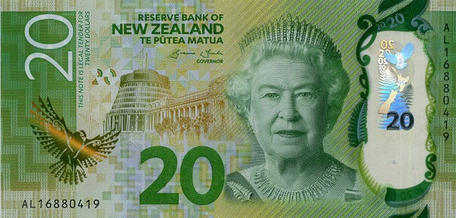
\includegraphics[width=0.6\textwidth,height=0.15\textheight]{../../pictures/images/nz20.png}
\caption{A 20 NZD note.}
\end{figure}

\begin{figure}[h!]
\centering
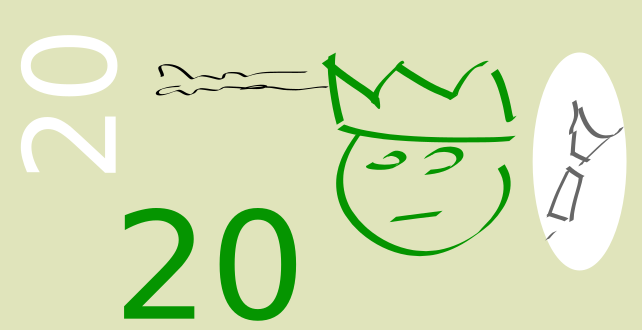
\includegraphics[width=0.6\textwidth,height=0.15\textheight]{../../pictures/drawings/my-nz20.png}
\caption{An artist's abstract rendering. This state abstraction only shows the essential details; $20$, New Zealand, ...}
\end{figure}

\newpage
\paragraph{Action abstraction} groups together 'similar' actions. For
example, both action $i$ and action $j$ might yield the same rewards and change in state,
in which case, we can just relabel them as the same action.

\begin{figure}[h!]
\centering
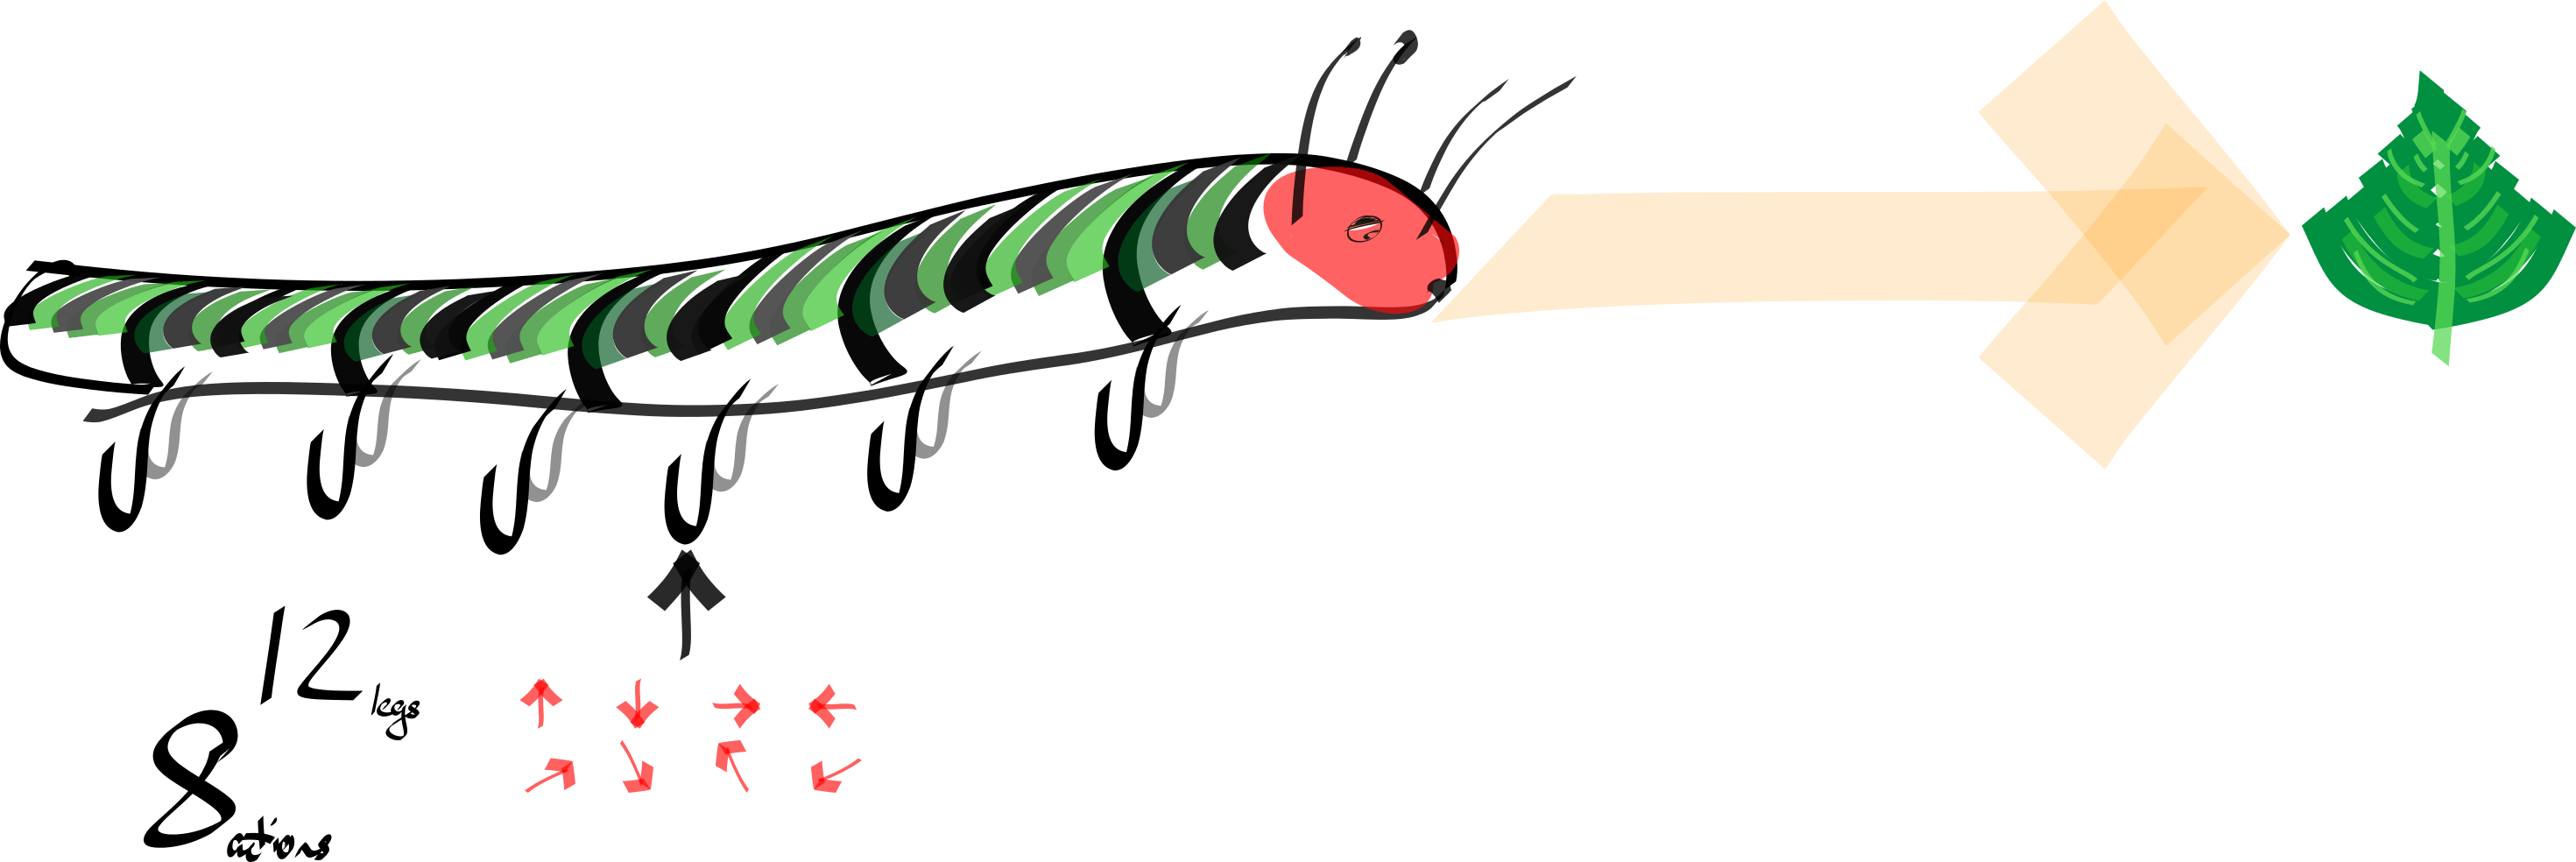
\includegraphics[width=0.7\textwidth,height=0.15\textheight]{../../pictures/drawings/hungry-caterpillar.png}
\caption{Consider a hungry caterpillar. It wants to move towards the leaf.
But this is a complicated task! Move your 3rd leg up, your 7th leg down, 11th leg slightly forward, etc...
To specify an action it needs to pick from $8^{12}$ possible actions - 8 actions per leg, 12 legs.}
\end{figure}


\begin{figure}[h!]
\centering
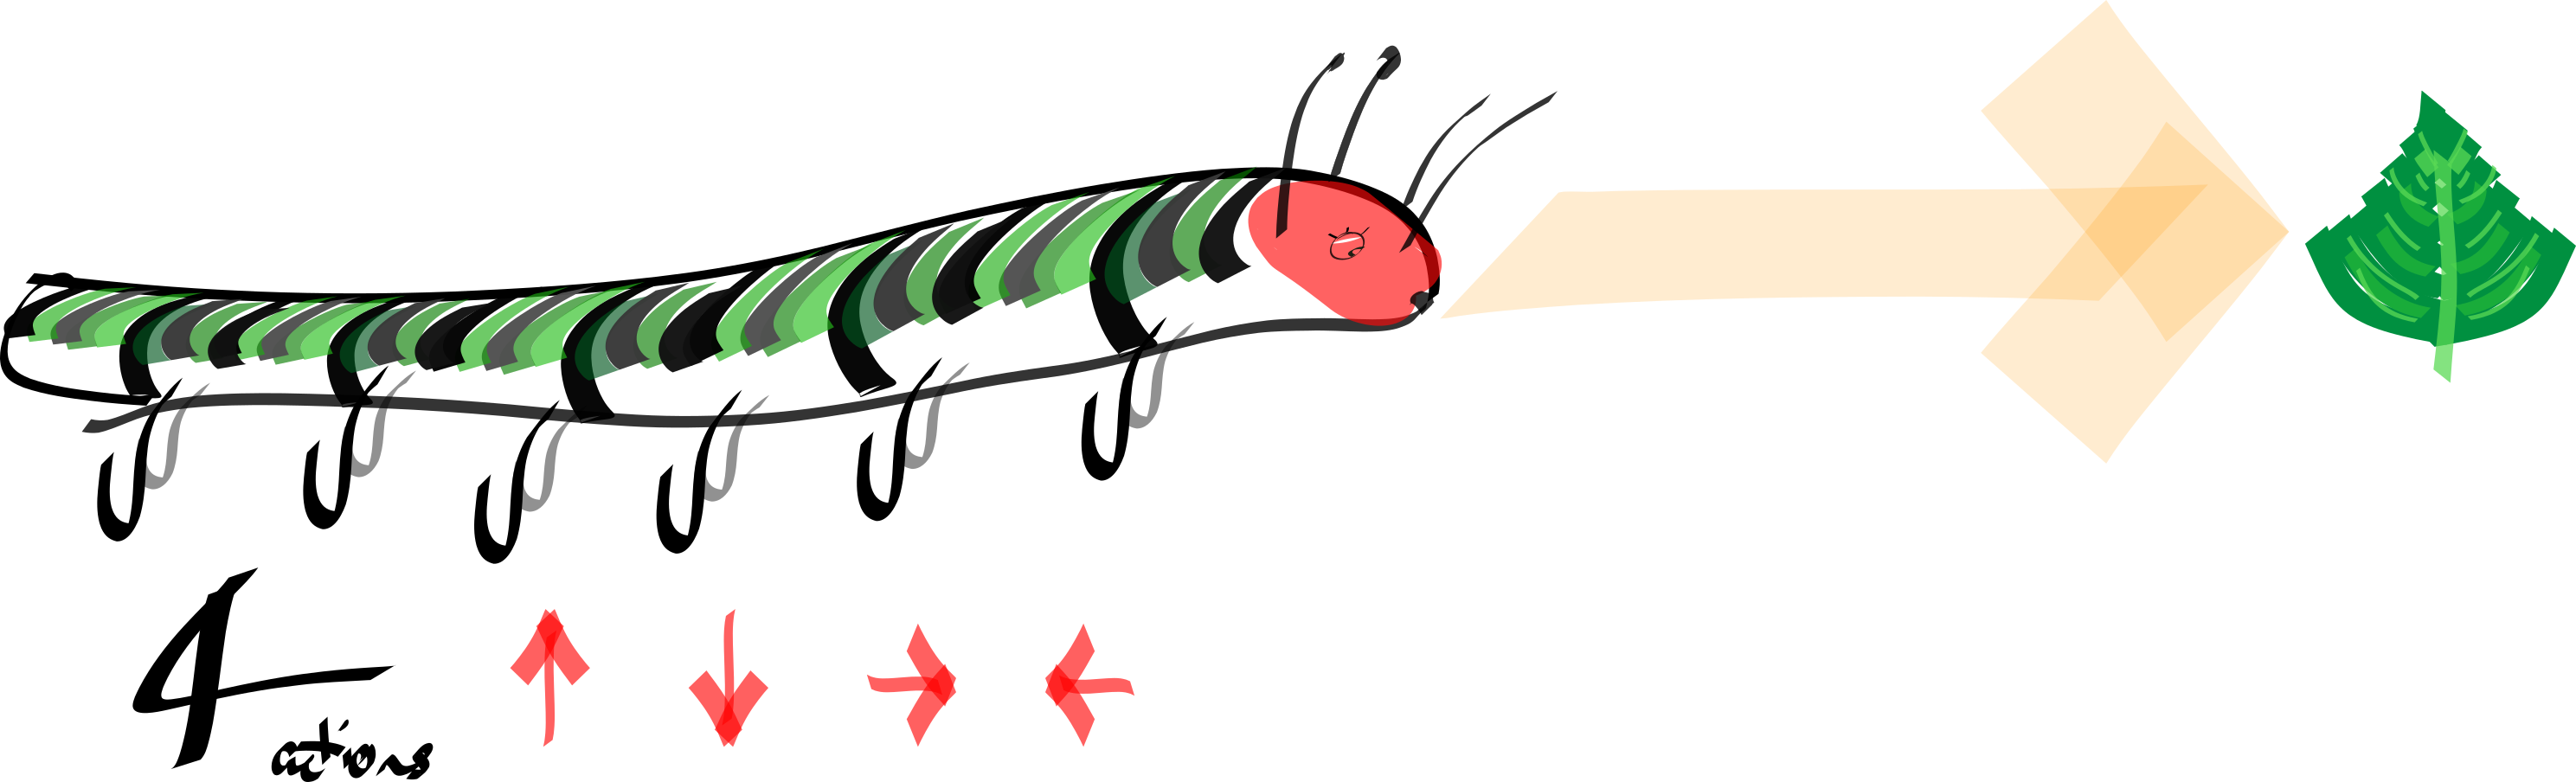
\includegraphics[width=0.7\textwidth,height=0.15\textheight]{../../pictures/drawings/full-caterpillar.png}
\caption{But, what if the caterpillar could specify actions in another way? Rather than specifying leg movements, it could pick a direction to move, which would specify the movement of multiple legs. Note, we are not including any temporal abstraction here.}
\end{figure}

\paragraph{State-action abstraction} groups together 'similar' state-actions.
This class of abstraction should be more powerful than state and action abstraction. Consider a mirror symmetric maze.

\begin{figure}[h!]
\centering
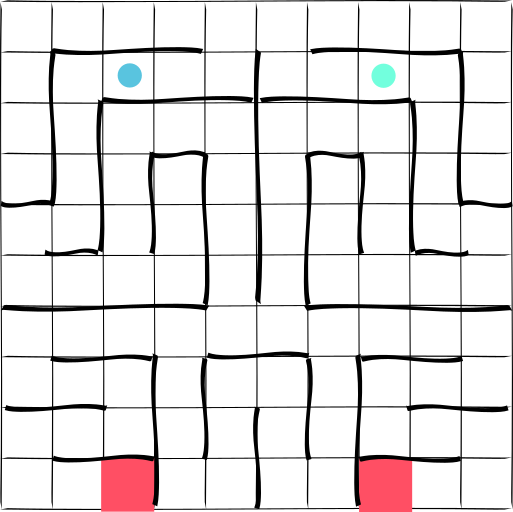
\includegraphics[width=0.75\textwidth,height=0.3\textheight]{../../pictures/drawings/maze.png}
\caption{A symmetric maze, the goal(s) are shown in red.
Consider two different, but 'similar' positions, shown in blue and green.}
\end{figure}

Given this setting, we can construct a representation of the state \footnotemark[11] where,
we have $Q^{\pi}(s, a) = Q^{-\pi}(-_xs, -a), \forall \pi$.
Where the negative operator $-_x$ only effects the horizontal ($x$) axis $s = (x, y), -_xs = (-x, y)$.
And $-\pi := \pi(-a|-_xs)$. \footnotemark[21]

\footnotetext[21]{The tradeoff is that with state-actions, now we need to keep track of $(|S| \times|A|)\cdot (|S| \times|A| - 1)$
similarities, rather than $|S|\cdot(|S|-1) + |A|\cdot(|A|-1)$ similarities.}

\footnotetext[11]{To construct this representation, we set the state to be centered around the mirror plane.
So the blue player is at location $(-3, 9)$ and the green player is at location
$(3, 9)$. And we equip the players with the actions $(+1, 0), (-1, 0), (0, -1), (, +1)$ (aka; up, down, left, right).}

State abstraction would not be able to group together the blue and green positions.
As moving left from blue is not equivalent to moving left from green.

\paragraph{Temporal abstraction} groups together 'similar' goals / options.
For example, the pumpkin recipe above: for the many ways there are to boil broth
(in pot, in a jug, over a wood fire, in the oven, ...), group them together.
For the many ways to puree pumpkin (with a rolling pin and some vigour, with a blender, ...), group them together.

The intuition behind both goal-like and option-like temporal abstractions is that
we can decompose a sequential decision problem into a set of shorter, easier to solve, parts.

\subsection{Discovering abstractions}

\begin{displayquote}
  \textit{Where do abstractions come from?}
\end{displayquote}

Earlier, we considered how an agent might use a given abstraction.
But where did that abstraction come from? Did someone construct it?
Or can abstractions be discovered automatically?

To build an abstraction, you need a notion of how two objects might be
similar (or a notion of what it is you want to preserve).
This allows you to group the 'similar' objects together, building an abstraction.
In RL there are many possible notions of similarity. But which ones are sensible?
Which ones allow us to efficiently finding the optimal policy?

\vspace{5mm}

\subsubsection{Classes of similarity for RL}\label{similar-classes}

Li et al. \cite{Littman2006} give five classes of state abstraction in which they group states based on various similarities \footnotemark[20];
\footnotetext[20]{Similarity and preservation are dual notions. Similarity tells us which objects we can group together,
'preservation' tells us which objects we group together to preserve (for lack of a better word...) a notion of similarity.
For example, the \textit{"preservation of the one step model"} means: two states can be considered similar if they have the same one step model.}

\textit{intuitively,
$\phi_{\text{model}}$ preserves the one step model,
$\phi_{Q_{\pi}}$ preserves the state-action value function for all policies,
$\phi_{Q^{* }}$ preserves the optimal state-action value,
$\phi_a^{* }$ preserves the optimal action and its value,
$\phi_{\pi^{* }}$ preserves the optimal action.}

\vspace{5mm}

We can construct a family of similarity functions for building abstractions for RL. To do so, we measure the
similarity between two 'RL objects'\footnotemark[28] as: for $x$ and $x'$,
how similar are their likely futures starting from those objects, for a range of different policies.
Let's make this formal.

\footnotetext[28]{Where RL objects could be one of; states, actions, state-actions, action-rewards, or state-action-rewards, ...}

Let $c(s, a, r)$ be a cumulant, and let $C$ be the expected discounted sum of that cumulant under a given policy
(where the exceptation is over all trajectories starting from $x$).\footnotemark[29]

\footnotetext[29]{This is also know as a general value function \cite{White2015}}

\begin{align*}
C(\zeta) &= \sum_{t=0}^{\infty} \gamma^{t}  c(\zeta_{t+1}) \\
\mathcal C(x, \pi) &= \mathop{\mathbb E}_{\zeta \sim D(\cdot | \pi, \zeta_{x})} [C(\zeta)] \\
\chi(x, x') &= \int_{\pi \in B} \frac{1}{1+\parallel \mathcal C(x, \pi) - \mathcal C(x', \pi) \parallel_{p}} d\pi
\end{align*}

We have written: the similarity $\chi$ between $x$ and $x'$ is; the sum over different policies, of the
similarities (the inverse of distance) between likely futures, starting from $x$ / $x'$.

 by setting $\zeta_x = {\zeta: \zeta_0^s = x^s, \zeta_0^a = x^a \forall \zeta \in \mathcal Z}$

{\color{red}HELP!?}

% Characterisation: How will we characterise these objects? By considering n-step futures, their expected value versus a rollout \footnotemark[9],
% \footnotetext[9]{These can be unified using the $Q(\sigma)$ algorithm \cite{Asis2018}}

\paragraph{Examples}

% Need to show that this family caputres abstrations of interest.
It would be nice to show that all abstractions of interest to RL live in this happy family.
Instead we will consider two abstractions. One abstraction constructed by preserving the n-step model,
and the other is constructed by preserving the value of the optimal state-actions.

\begin{itemize}
  \tightlist
  \item Preserving the n-step model: We start with $x=(s, a), x'=(s', a')$. Set $c(\zeta_{t}) = [s_{t+1}, r_{t}]$ then $\mathcal C=[N, V]$, where $N$ is the discounted state visitation count \footnotemark[27] and $V$ is the state value. Two $x$s with the same state visitation and value for all policies must have the same transitions. {\color{red}(need to prove?!?)}
  \item Preserving the optimal state-action value: Again, we start with $x=(s, a), x'=(s', a')$. Next, we pick $c(\zeta_{t}) = r_{t}$ which means $\mathcal C(x, \pi) = Q^{\pi}(s, a)$.
\end{itemize}

\footnotetext[27]{If we have encoded the states as onehots.}

\subsubsection{Inference of the similarity}

\begin{displayquote}
	\textit{How might we infer that two objects are similar?}
\end{displayquote}

% So we have our measure of similarity. But we need data.
% We want these masures of similarity to generalise. How? Priors.

In the RL setting, we are often not given the transition or the reward function.
Thus, we must infer similarities from noisy observations. There are two ways we can do this;

\hspace{\parindent}We can infer that two objects are similar because we have seen it,
we have sufficient data (/ experience) to allow us to conclude that, with high
certainty, $x_i$ and $x_j$ are similar (with probability $\delta$, $f(x_i) - f(x_j) \le \epsilon$ ).

\hspace{\parindent}Alternatively, we can infer that two objects are similar because we have found a pattern.
For example, we might have seen that rotations of $45, 90, 135$$, 180, 225$, are all similar,
therefore we guess that rotations of $270, 315$ are also similar.
This motivates our work on symmetric abstractions \ref{symmetric-abstractions}.
Because of the structure in a symmetry, a similarity can imply others. And thus we can generalise.

Note: if we are relying on inferring similarity from data, and $f(x_i) = Q^{\pi^{* }}(s_i, a_i)$.
Then learning that $x_i$ and $x_j$ are similar doesn't really help us.
To estimate that similarity we had to know, $Q^{\pi^{* }}(s_i, a_i)$ and $Q^{\pi^{* }}(s_j, a_j)$.
Rather, we care about (correctly) guessing that $x_i$ and $x_j$ are similar, so we can
use the knowledge that $Q_i = Q^{\pi^{* }}(s_i, a_i)$ to help us learn $Q^{\pi^{* }}(s_j, a_j)$.

\subsection{Evaluating abstractions}

\begin{displayquote}
\textit{But.
Which class of abstraction should we use?
Which class of similarity measure should we use?
We need to be able to evaluate these.}
\end{displayquote}

Ideally we would pick the most 'coarse' abstraction, as a coarse abstraction means we have grouped together many objects.
Thus it has potential for the greatest increases in computational and sample efficiency.
But. Coarseness is not the only property of an abstraction we care about.
An abstraction must also allow us to represent near optimal policies and it must allow us
to efficiently find those near optimal policies.

Ideally, we would be able to summarise the 'coarseness', 'sub-optimality' and 'efficiency' all in a single number.
Then we could try to optimise it. But for now, let's define these constraints on 'good' abstractions.

\subsubsection{Coarse abstractions}

% related to compression?
% also heirarhical abstractions?! related to multiple layers of abstraction of different coarseness?!

Coarse (as opposed to fine) is a notion from topology.
A (more) coarse abstraction describes an abstraction that has a looser
notion of similarity (more things are considered similar). \footnotemark[24]

\footnotetext[24]{(Coarseness captures concepts such as a 'high level' abstraction or a 'general' abstraction).}

\textit{We say [state abstraction] $\phi_2$ is coarser than [state abstraction] $\phi_1$, denoted $\phi_1 \ge \phi_2$,
iff for any states $s_1, s_2 \in S, \phi_1(s_1) = \phi_1(s_2)$ implies $\phi_2(s_1) = \phi_2(s_2)$.} \cite{Littman2006}

Any time $s_1$ and $s_2$ are considered similar in an abstraction, then a coarser
abstraction will also consider them to be similar, and there might also be other similar states. \footnotemark[25]

\footnotetext[25]{So the most coarse abstraction would be where everything is mapped to the same abstract state.
$\forall s_i, s_j\in S: \phi(s_i)=\phi(s_j)$.}

\begin{displayquote}
\textit{Why are coarse abstractions desirable?}
\end{displayquote}

By throwing away inessential details;
\begin{itemize}
  \tightlist
  \item there is less to compute.
  \item we will not waste time exploring them.
  \item we have reduced the variance of our observations and thus allow quicker learning.
\end{itemize}

These arguments have been formalised in the case of symmetries and are described in \ref{symmetric-exploitation}.

% reduce variance in estimates   \cite{Allen-Zhu2016a,Johnson2013a}
  % take size of smallest partition to be X. use this to say: reduces variances by at least a factor of X.
% spend less time exploring unimportant states / actions
  % in the ?? abstraction case.

\subsubsection{Near optimal abstractions}

Imagine we have a state abstraction, a road is a road, there is no real difference
between them; gravel, winding, motorway, cliffs-on-either-side...
One of the first things we want to know about the abstraction is:
is it possible for me to act optimally
using this abstraction? If not, what's the damage? In this case, does driving 100kph on every road --
because they are all pretty-much-the-same -- lead to suboptimal results? Probably.
More precisely, we want know to whether the optimal policy can be approximately represented within an abstracted MDP.

% formal
This notion of near-optimality (aka sub-optimality) can be formalised as the representation error of the optimal
policy. \cite{Abel2017} Given an abstraction, we want to know how well the abstraction can represent the optimal policy.

\begin{align}
\forall_{s\in S} \mid V^{\pi^* }(s) - V^{\pi_{A}^* }(s) \mid \le \epsilon
\end{align}

Where $\pi^{* }$ is the optimal policy, and $\pi_{A}^{* }$ is the lifted optimal
policy found using the abstraction.

This notion can be generalised to other types of abstraction, for example
Nachum et al. 2018 \cite{Nachum2018} extend this concept of near optimal
representation of the optimal policy to goal-like temporal abstraction. \footnotemark[13]

\footnotetext[13]{To do this, Nachum et al. 2018 \cite{Nachum2018} quantify
how many of the possible low level behaviours can be produced by different choices of goal.
This is roughly a measure of the invertability of the 'low level' policy from
state-goals to temporally extended actions.
This allows them to reason about which behaviours are representable using goals,
and thus whether a 'high level' policy choosing these goals can approximate the optimal policy.}

\subsubsection{Efficiently solvable abstractions}

Just because a near optimal policy exists (under our abstraction), that does not mean it will be easy to find.
We might require large amounts of data or computation.

\paragraph{Efficient control:} \textit{What is needed for efficient control. And when is 'it' preserved?}

We want to preserve our ability to use the Bellman equation to efficiently guide the search for optimal controls.
But, what is necessary or sufficient to preserve the Bellman equation's ability to guide search?

\begin{displayquote}
\textbf{Claim:} Preserving the value of the optimal action is sufficient to preserve the Bellman equation's ability to guide search.
\end{displayquote}

% If we have preserved the value of the optimal action (for each action), then, for all actions $\forall a: Q(s, a) \le Q(s, a^{* })$.
Consider an abstraction that has preserved the value of the optimal action.
When constructing the abstraction, we may have grouped together states that dont have similar transitions, or similar value under all policies, ... etc.
For example we might have: $s_i \sim s_j$ despite $Q(s_i, a_k) - Q(s_j, a_k) > \epsilon, a_k \neq a^{* }$.
But this doesnt matter as $Q(s, a^{* })$ must still be larger than $Q(s, a_k)$.
Thus, when applying a greedy update to the Bellman equation, we are going to converge
\footnotemark[26]

{\color{red}but the new Q values might change the topology of the problem?!?!}

\footnotetext[26]{This argument needs to be formalised. So far, we only have empirical evidence of this. Also, related work has shown that if the value of the optimal action is not preserved then applying the Bellman equation no longer guarantees that optimal policies are also optimal in the abstraction. \cite{Jong2005}}

\paragraph{Efficient exploration:} \textit{What is needed for efficient exploration. And when is 'it' preserved?}

For $Q$-learning, Jin el at. \cite{Bubeck2018} show that efficient exploration ($\mathcal O(\sqrt{H^3SAT})$)\footnotemark[13] can be
achieved with a UCB-Bernstein type exploration bonus, compared to the inefficient exploration ($\mathcal O(\sqrt{H^4SAT})$),
achieved by the UCB-Hoeffding type exploration bonus. To achieve this, the UCB-Bernstein type exploration bonus needed to incorporate an
estimate the variance of the values, while the Hoeffding exploration bonus relies only on visitation counts.

\footnotetext[13]{$\mathcal O(\sqrt{H^3SAT})$ tells us that the expected regret scales, in the worst case, as a function of $\sqrt{H^3SAT}$.
Where $H$ is the planning horizon, S is the size of the state space, $A$ is the size of the action space and $T=KH$, where $K$ is the total number of episodes played.}

This tells us that, if we want to preserve our ability to efficiently explore (in the sense above) we need to preserve the  ability to accurately estimate the variance of the value function.

% If the value under the abstraction of even a single state is wrong, it could arbitrarily change the variance estimates
% (well, that isnt true...?!? depends on the value of the other states we might share with)

% Is this true in general, or specific to Q-learning with exploration bonuses? Future work.

\paragraph{Efficient inference:} \textit{What is needed for efficient inference. And when is 'it' preserved?}

% What are we hoping to infer efficiently? In this case. The model parameters. Or the value of a state-action?

\cite{Allen-Zhu2016a,Johnson2013a}
% these refs actually show faster convergence not faster learning!?

% Alternatively could frame as ERM for model params!?

% \begin{align*}
% \text{Regret()} = \mathbb E [\sum V^{\pi^{* }}() - V^{\pi}]
% \end{align*}

{\color{red}TODO}

% \begin{center}\rule{0.5\linewidth}{\linethickness}\end{center}
%
% So, now that we have a notion of better / worse abstractions. Let's consider the abstractions
% that Li et al. \cite{Littman2006} defined.
%
% Li et al. \cite{Littman2006} show that $\phi_G \le \phi_{\text{model}} \le \phi_{Q_{\pi}} \le \phi_{Q^{* }} \le \phi_a^{* } \le \phi_{\pi^{* }}$
%
% So we should prefer $\phi_{\pi^{* }}$? But.
% There exist examples where the optimal policy found using $\phi_{\pi^{* }}$ is not optimal in the ground MDP \cite{Jong2005}.
% So the best choice appears to be $\phi_a^{* }$.

\subsubsection{The complexity of abstraction}

We hope to build learners capable of discovering and exploiting an abstraction
to efficiently solve the problems they are given.
But, the efficiency gains of using an abstraction (as measured by its evaluation - in the above section) \underline{must} offset the cost of
discovering that abstraction! Else, why did we bother...?

\begin{displayquote}
\textit{"The challenge in the single-task case is overcoming the additional cost of discovering [an abstraction];
this results in a narrow opportunity for performance improvements, but a well-defined objective.
In the ... transfer case, the key challenge is predicting the usefulness of a particular [abstraction] to future tasks, given limited data.""}\cite{Konidaris2019}
\end{displayquote}

For arbitrary problems, as often as we guess right about "the best abstraction for this task" or "the usefulness of a particular abstraction to future tasks",
there will be another set of future tasks where we are wrong. This is a result of the no free lunch theorem \ref{Wolpert1996}. However, we can hope for good performance on restricted classes of problems.

To evaluate an abstraction for the single task case we need to compare the complexity of
finding a solution via abstraction (abstract, solve, lift) against the performance against
solvers that do not abstract.

In the transfer case, we need to construct a set of task. And accumulate the
complexity of discovering the abstraction, and the complexity of solving
and lifting the abstraction for each new task.

% \subsection{Related work: Representation learning for RL}
%
% % \begin{displayquote}
% %   \textit{[Abstraction] is a mapping from one problem representation to a new representation, while preserving some properties} (Littman / Walsh.)
% % \end{displayquote}
%
% {\color{red}There is a lot to talk about here...}
%
% Representations that attempt to preserve
% \begin{itemize}
% \tightlist
%   \item the mutual information between ? and ??.
%   \item knowledge required to predict the next state
%   \item ... geometric bellamere
%   \item \cite{Nachum2018}
%   \item autoencoders...
%   \item next step prediction.
% \end{itemize}
%
% But with what guarantees?
